\section{Bài toán nhận diện làn đường}
Trong bài toán lần này, nhóm sẽ đề xuất một giải thuật nhằm giúp xe phát hiện vị trí tương đối của bản thân chiếc xe và khoảng cách từ nó đến 2 vạch kẻ của làn đường. Mục đích của việc này là giúp xe có thể đưa ra những thông số về khoảng cách, độ lệch so với trung tâm hoặc phương hướng của làn đường (thẳng, cong) rồi từ đó bộ điều khiển sẽ tính toán và cân bằng ở chính giữa làn đường trong suốt thời gian di chuyển. Nhóm xin phép đề xuất một giải thuật như sau, tạm gọi là \textbf{giải thuật góc nhìn của chim (bird's eyes view algorithm)}. \\
\newline
Cụ thể, các bước cần thực hiện để hiện thực giải thuật như sau:
\begin{enumerate}
    \item \textbf{Hiệu chỉnh camera:}
    \begin{itemize}
        \item Sử dụng một tập hình ảnh bàn cờ vua chụp từ cùng một camera như ảnh đầu vào.
        \item Trả về tọa độ 4 góc của bàn cờ vua bằng các hàm của thư viện OpenCV.
        \item Sử dụng các góc phát hiện được để hiệu chỉnh camera và lấy ma trận hiệu chỉnh camera cùng các hệ số méo.
    \end{itemize}

    \item \textbf{Điều chỉnh méo ảnh:}
    \begin{itemize}
        \item Áp dụng ma trận hiệu chỉnh camera và các hệ số méo để sửa chữa méo ống kính trong ảnh gốc.
    \end{itemize}

    \item \textbf{Phân ngưỡng ảnh:}
    \begin{itemize}
        \item Sử dụng các biến đổi màu sắc, độ dốc và các kỹ thuật khác để tạo ra ảnh nhị phân dựa trên ngưỡng.
        \item Các phương pháp ngưỡng có thể bao gồm ngưỡng độ dốc, ngưỡng màu (ví dụ, trong không gian màu HLS hoặc LAB) và ngưỡng thích ứng.
    \end{itemize}

    \item \textbf{Biến đổi góc nhìn:}
    \begin{itemize}
        \item Áp dụng một biến đổi góc nhìn để có được "góc nhìn từ trên cao" của làn đường.
        \item Xác định các điểm nguồn và đích cho biến đổi góc nhìn.
        \item Sử dụng các hàm getPerspectiveTransform và warpPerspective của OpenCV.
    \end{itemize}

    \item \textbf{Phát hiện làn đường và điều chỉnh điểm làn:}
    \begin{itemize}
        \item Xác định điểm làn bằng cách sử dụng các kỹ thuật như đỉnh lịch sử hoặc cửa sổ trượt.
        \item Điều chỉnh một đa thức để biểu diễn biên giới của làn đường được phát hiện.
    \end{itemize}

    \item \textbf{Ước lượng độ cong làn đường:}
    \begin{itemize}
        \item Tính toán cong đường của làn đường được điều chỉnh bằng các công thức toán học phù hợp.
        \item Xác định vị trí của xe so với trung tâm của làn đường.
    \end{itemize}

    \item \textbf{Điều chỉnh làn trở lại:}
    \begin{itemize}
        \item Điều chỉnh biên giới của làn đường được phát hiện trở lại trên ảnh gốc bằng cách sử dụng biến đổi góc nhìn nghịch đảo.
    \end{itemize}

    \item \textbf{Hiển thị:}
    \begin{itemize}
        \item Xuất hiển thị hình ảnh của biên giới làn đường trên ảnh gốc bao gồm các ước lượng số liệu về đường cong và vị trí của xe.
    \end{itemize}
\end{enumerate}
\newline 
Như vậy, có thể hiểu đây là một quá trình chuyển đổi góc nhìn 2D từ camera quay trở lại điểm nhìn thật trong thế giới 3D thật vốn có. Trong giải thuật này, quá trình hiệu chỉnh camera là một bước quan trọng để khắc phục méo ảnh từ góc độ hình ảnh, đặc biệt là khi camera nhìn vào các đối tượng 3D trong thế giới thực và chuyển đổi chúng thành một ảnh 2D trên mặt phẳng hình ảnh. Méo ảnh có thể làm thay đổi hình dạng và kích thước của đối tượng trong quá trình này, ảnh hưởng đến khả năng nhận dạng làn đường.\\
\newline
Tóm tắt lại, ta có quy trình hiện thực giải thuật như sau:
\begin{figure}[htbp]
    \centering
    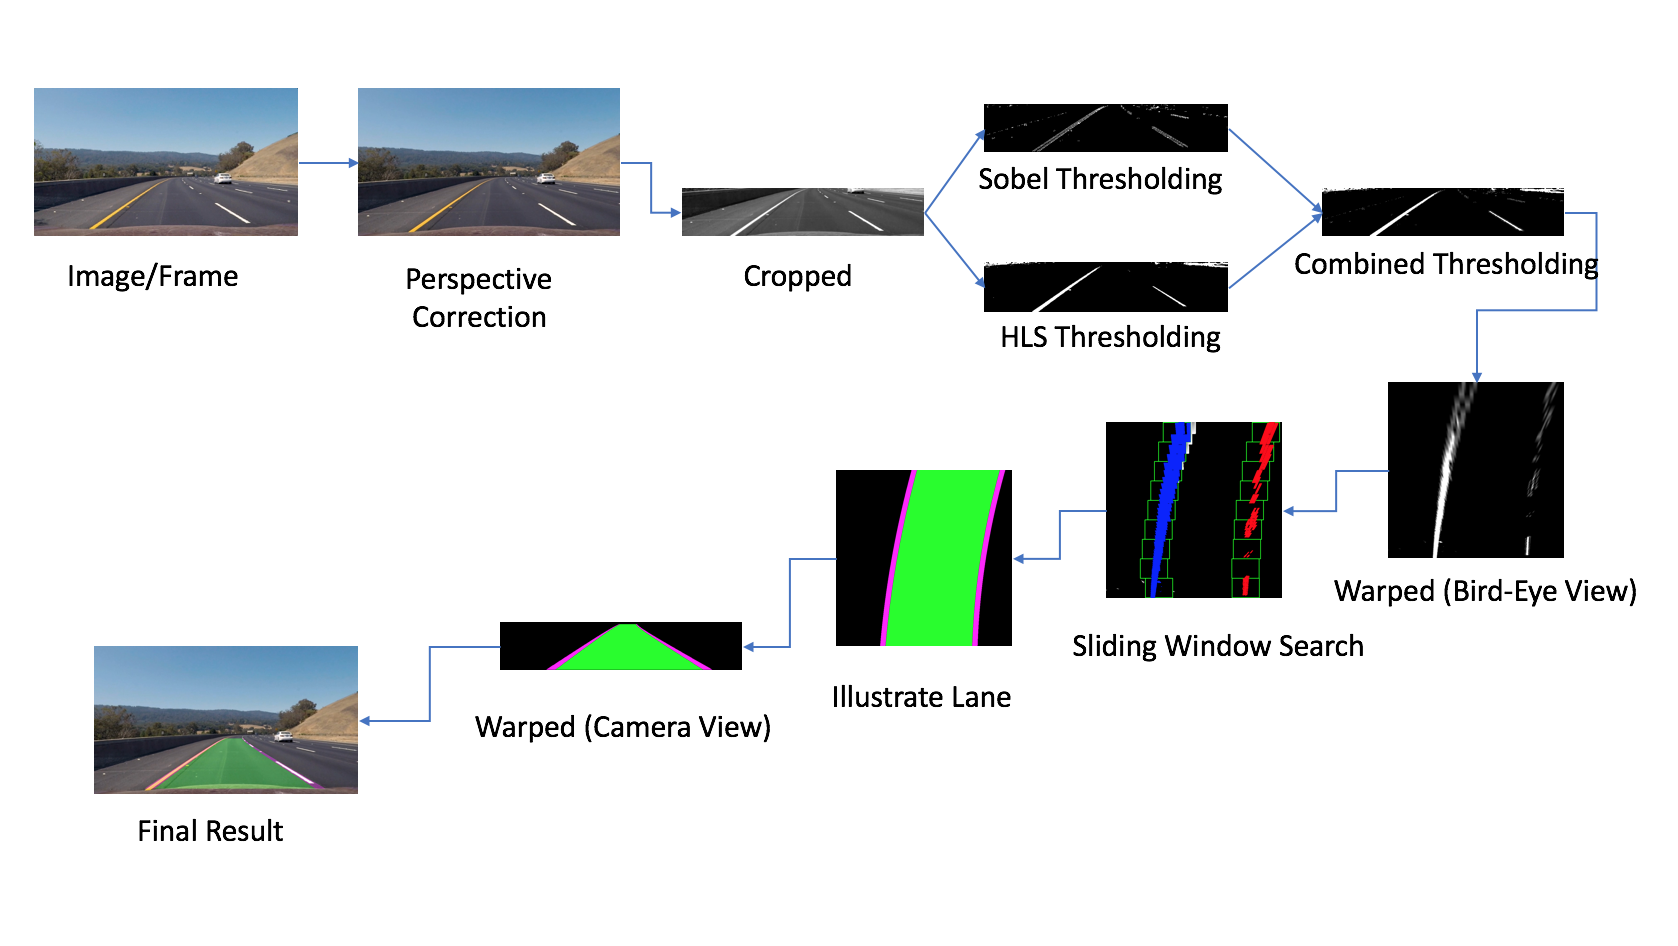
\includegraphics[width = 0.8\textwidth]{images/3-lane/pipeline.png}
    \caption{Bird's eyes view}
\end{figure}
\newline 
Sau đây, ta sẽ đi sau hơn vào từng phần đồng thời giải thích rõ hơn phương pháp và giải thuật mà nhóm đang sử dụng.

\subsection{Hiệu chỉnh camera (camera calibration)}
Quá trình chụp ảnh thông qua ống kính có thể tạo ra sự méo lệch đáng kể trong hình ảnh. Có hai loại méo lệch chính, đó là méo lệch tâm cầu và méo lệch tiếp xúc. Hiện tượng méo ảnh xảy ra khi camera quan sát các đối tượng có đặc tính 3D trong thế giới thực và muốn chuyển chúng thành mặt phẳng 2D trên ảnh. Thực tế, quá trình chuyển đổi này không thể hiệu quả và gây ra nhiều méo ảnh trong hình ảnh, làm thay đổi hình dạng và kích thước của đối tượng trong quá trình chuyển đổi. Do đó, việc đánh giá mức độ méo ảnh của hình ảnh được coi là bước tiền xử lý quan trọng. Thực tế, bước này ảnh hưởng đáng kể đến hiệu suất của việc phát hiện làn đường, vì hình ảnh bị méo sẽ làm cho làn đường trong một số phần trở nên cong và đưa ra khỏi ứng dụng phát hiện từ thực tế. Nó cũng làm cho hình ảnh trông nghiêng, khiến cho một số đối tượng trông xa hơn hoặc gần hơn so với thực tế.
\newpage
\begin{figure}[htbp]
    \centering
    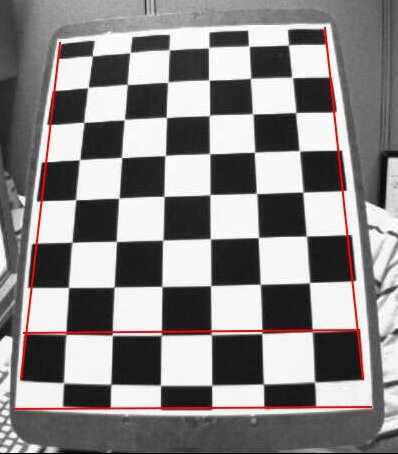
\includegraphics[width = 0.4\textwidth]{images/3-lane/calib_radial.jpg}
    \caption{Hiện tượng lệch ảnh}
\end{figure}
Trong đó:
\begin{itemize}
    \item (x,y) là tọa độ của một điểm trong hình ảnh bị méo.
    \item $(x_{distorted},y_{distorted})$ là tọa độ tương ứng của điểm đã được làm phẳng sau khi được sửa chữa.
    \item r là khoảng cách từ trung tâm của hình ảnh đến điểm (x,y).
    \item $k_1, k_2, k_3$ là các hệ số méo lệch tâm cầu xác định mức độ méo lệch tâm cầu.
\end{itemize}
\noindent Độ méo lệch tâm cầu có thể được biểu diễn như sau:
\begin{equation*}
    \begin{aligned}
        x_{distorted} &= x(1 + k_1 r^2 + k_2 r^4 + k_3 r^6)\\
        y_{distorted} &= y(1 + k_1 r^2 + k_2 r^4 + k_3 r^6)
    \end{aligned}
\end{equation*}

\noindent Tương tự, méo lệch tiếp xúc xảy ra vì ống kính chụp ảnh không được căn chỉnh hoàn hảo song song với mặt phẳng hình ảnh. Do đó, một số khu vực trong hình ảnh có thể trông gần hơn so với dự kiến. Số lượng méo lệch tiếp xúc có thể được biểu diễn như sau:
\begin{equation*}
    \begin{aligned}
        x_{distorted} &= x + [2 p_1 x y + p_2(r^2 + 2x^2)]\\
        y_{distorted} &= y + [p_1 (r^2 + 2 y^2) + 2 p_2 x y]
    \end{aligned}
\end{equation*}

\noindent Tóm lại, chúng ta cần xác định năm tham số, được gọi là các hệ số méo lệch, theo công thức:
\begin{center}
    Distortion coefficients = ($k_1$, $k_2$, $p_1$, $p_2$, $k_3$)
\end{center}

\noindent Tiêu cự và quang tâm có thể được sử dụng để tạo ra ma trận camera, từ đó có thể loại bỏ méo lệch do ống kính của một camera cụ thể. Ma trận camera là duy nhất đối với một camera cụ thể, vì vậy khi tính toán một lần, nó có thể được sử dụng lại trên các hình ảnh khác chụp bởi cùng một camera. Ma trận này được biểu diễn dưới dạng ma trận 3 x 3: 
\[
Camera Matrix = 
\left[
\begin{array}{ccc}
    f_x & 0 & c_x \\
    0 & f_y & c_y \\
    0 & 0 & 1
\end{array}
\right]
\]
Các bước thực hiện hiệu chỉnh ảnh như sau:
\begin{enumerate}
    \item Chuẩn bị "điểm vật", là các tọa độ (x, y, z) của các góc của bảng cờ vua trong thế giới thật. Điều này giả sử bảng cờ vua được cố định trên mặt phẳng (x, y) ở z = 0. Đồng thời, giả sử kích thước của mô hình bảng cờ vua giống nhau cho tất cả các hình ảnh, nên "điểm vật" sẽ giống nhau cho mỗi hình ảnh hiệu chỉnh.
    \item Tiếp theo, hình ảnh hiệu chỉnh được nạp tuần tự, chuyển đổi sang ảnh xám (gray scale), và tìm kiếm mô hình bảng cờ vua bằng \textbf{cv2.findChessboardCorners}. Khi mô hình được tìm thấy, vị trí của các góc được làm sáng cường thêm để đạt được độ chính xác sub-pixel bằng cách sử dụng \textbf{cv2.cornerSubPix}. Điều này nâng cao độ chính xác của hiệu chỉnh. Tọa độ của góc được thêm vào danh sách chứa tất cả các điểm ảnh, trong khi "đối tượng" được chuẩn bị được thêm vào danh sách chứa tất cả các "điểm vật".
    \item Hệ số méo (distortion coefficients )và ma trận camera (camera matrix) được tính toán bằng cách sử dụng hàm \textbf{cv2.calibrateCamera()}, trong đó hình ảnh và điểm "đối tượng" được chuyển làm đầu vào. Quan trọng là kiểm tra xem kết quả có đạt được không, vì hiệu chỉnh là một quy trình số học phi tuyến tính, nên nó có thể tạo ra kết quả không tối ưu. Để làm điều này, hình ảnh hiệu chỉnh được đọc một lần nữa và đưa ra sự méo ảnh. Hình ảnh đã được làm phẳng được hiển thị để kiểm tra mắt xem sự méo ảnh đã được sửa chữa hay chưa. Sau khi dữ liệu đã được kiểm tra, các tham số được đóng gói và lưu vào tệp. Một ví dụ về hình ảnh đầu vào, hình ảnh với góc của bảng cờ vua và hình ảnh đã được làm phẳng được hiển thị.
\end{enumerate}
\begin{table}[h]
    \centering
    \begin{tabular}{|c|c|c|}
        \hline
        \rowcolor[gray]{0.9}
        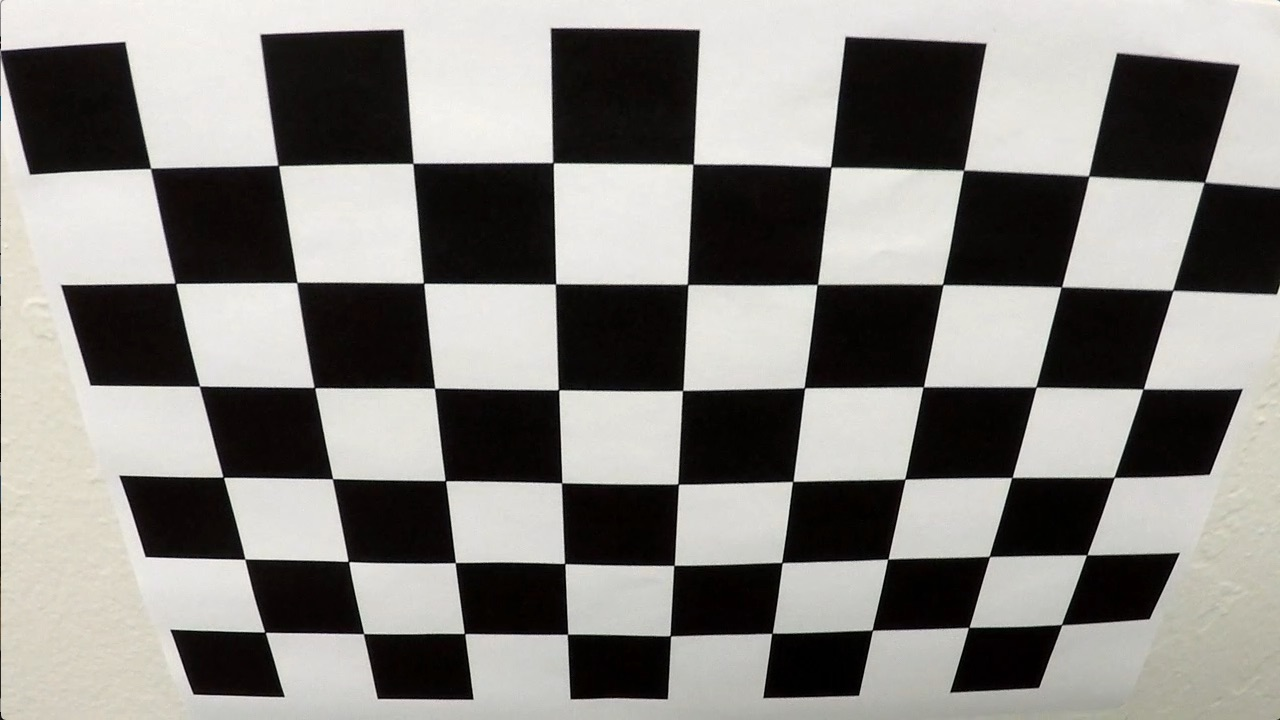
\includegraphics[width=0.3\linewidth]{images/3-lane/o.jpg} & 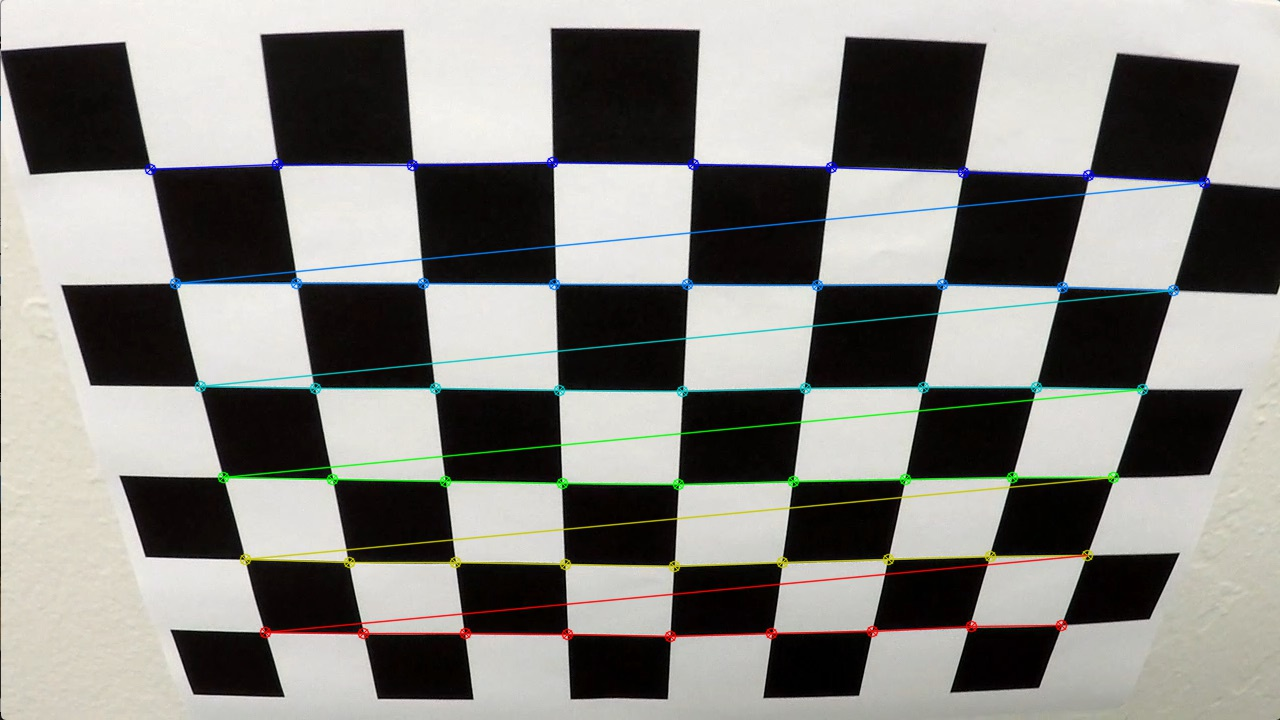
\includegraphics[width=0.3\linewidth]{images/3-lane/c.jpg} & 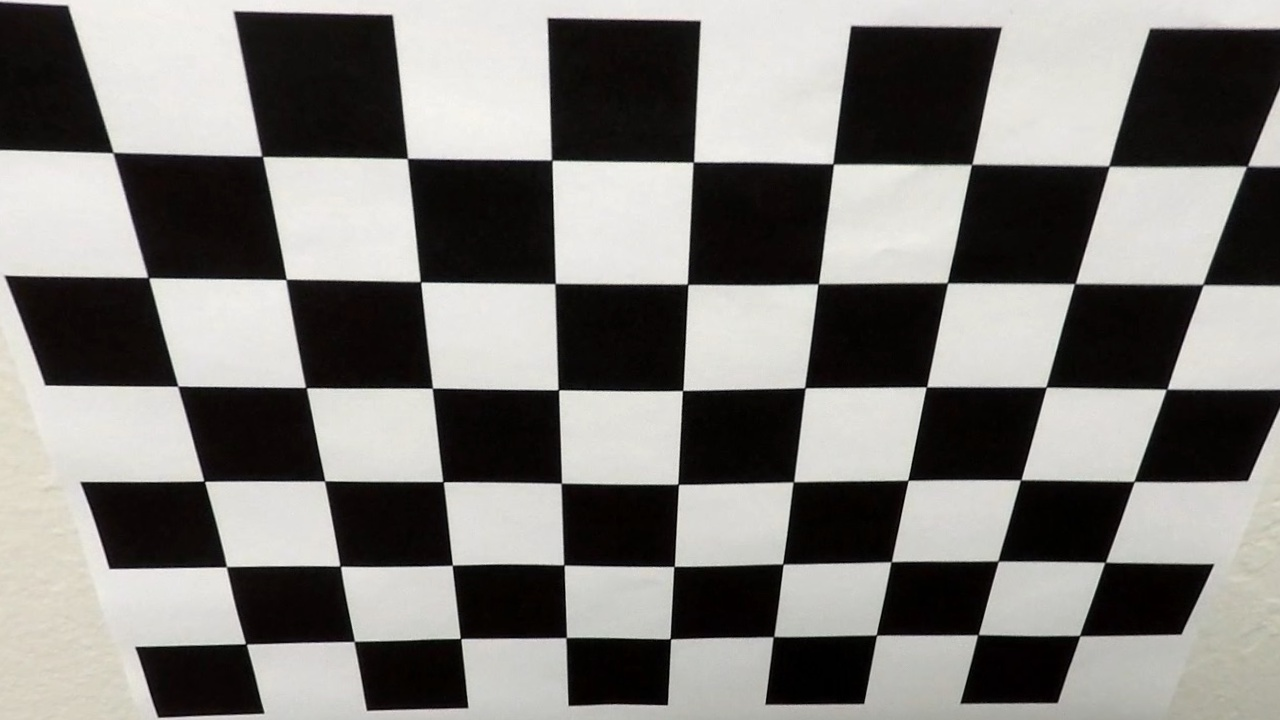
\includegraphics[width=0.3\linewidth]{images/3-lane/u.jpg} \\
        \hline
        \rowcolor[gray]{0.9}
        \textbf{Original image} & \textbf{Chessboard corners} & \textbf{Undistorted image} \\
        \hline
        \rowcolor[gray]{0.9}
    \end{tabular}
        \caption{Hiệu chỉnh ảnh trên bàn cờ vua}
\end{table}

\noindent Ma trận camera bao gồm mô hình camera "lỗ khóa" (pinhole) trong đó. Nó cung cấp mối quan hệ giữa tọa độ của các điểm liên quan đến camera trong không gian 3D và vị trí của điểm đó trên hình ảnh theo đơn vị pixel. Nếu X, Y và Z là tọa độ của điểm trong không gian 3D, vị trí của nó trên hình ảnh (u và v) theo đơn vị pixel được tính bằng cách sử dụng:
\newline
\begin{equation*}
    \begin{aligned}
        \left[
    \begin{array}{c}
    \\
         u  \\
         v  \\
         1
    \end{array}   
\right]
&= sM
\left[
    \begin{array}{c}
    
         X  \\
         Y  \\
         Z
    \end{array}   
\right]
    \end{aligned}
\end{equation*}
Trong đó M đại diện cho ma trận camera, và ss là một hệ số vô hướng khác không bằng không. Phương trình này sẽ được sử dụng sau này.
\newpage
\subsection{Áp dụng hiệu chỉnh ảnh}
Áp dụng hiệu chỉnh ảnh, ta thu được hình ảnh trước và sau khi sử dụng trên như sau:
\begin{figure}[htbp]
    \centering
    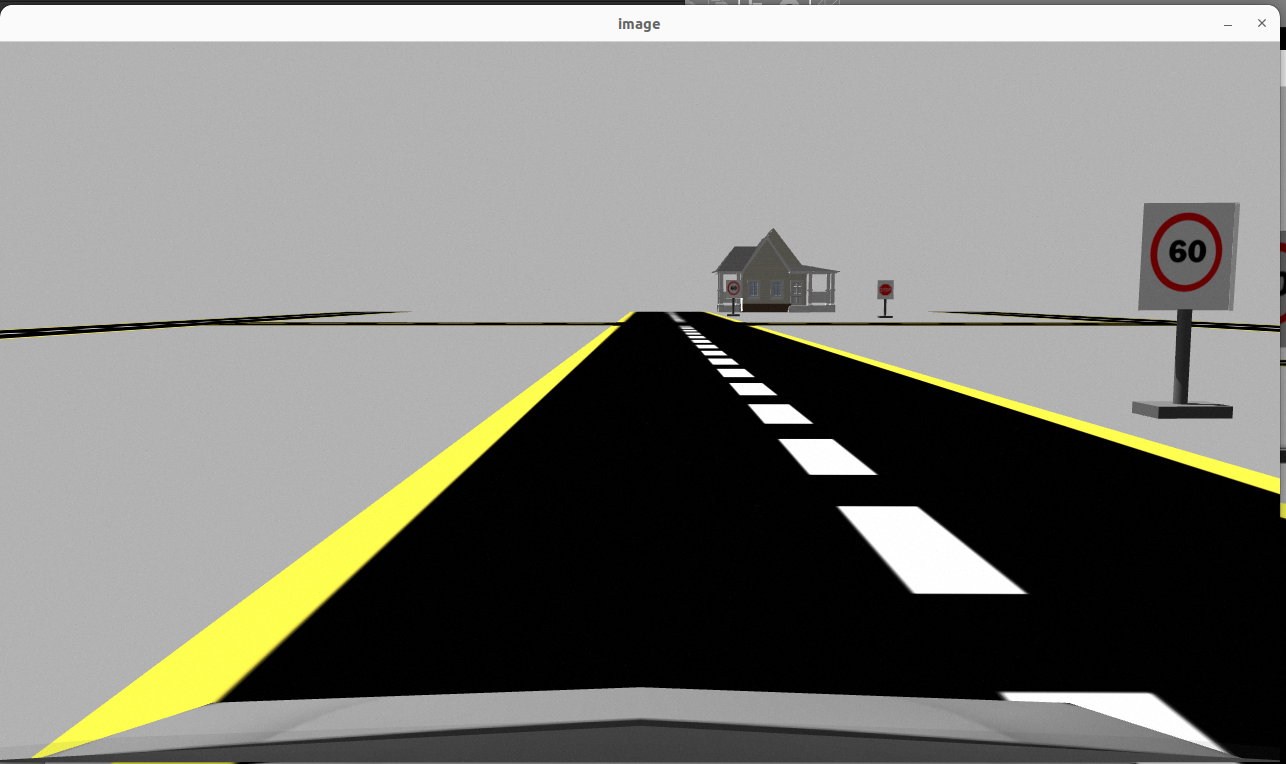
\includegraphics[width=0.6\linewidth]{images/3-lane/d._img.png}
    \caption{Trước hiệu chỉnh}
\end{figure}
\begin{figure}[htbp]
    \centering
    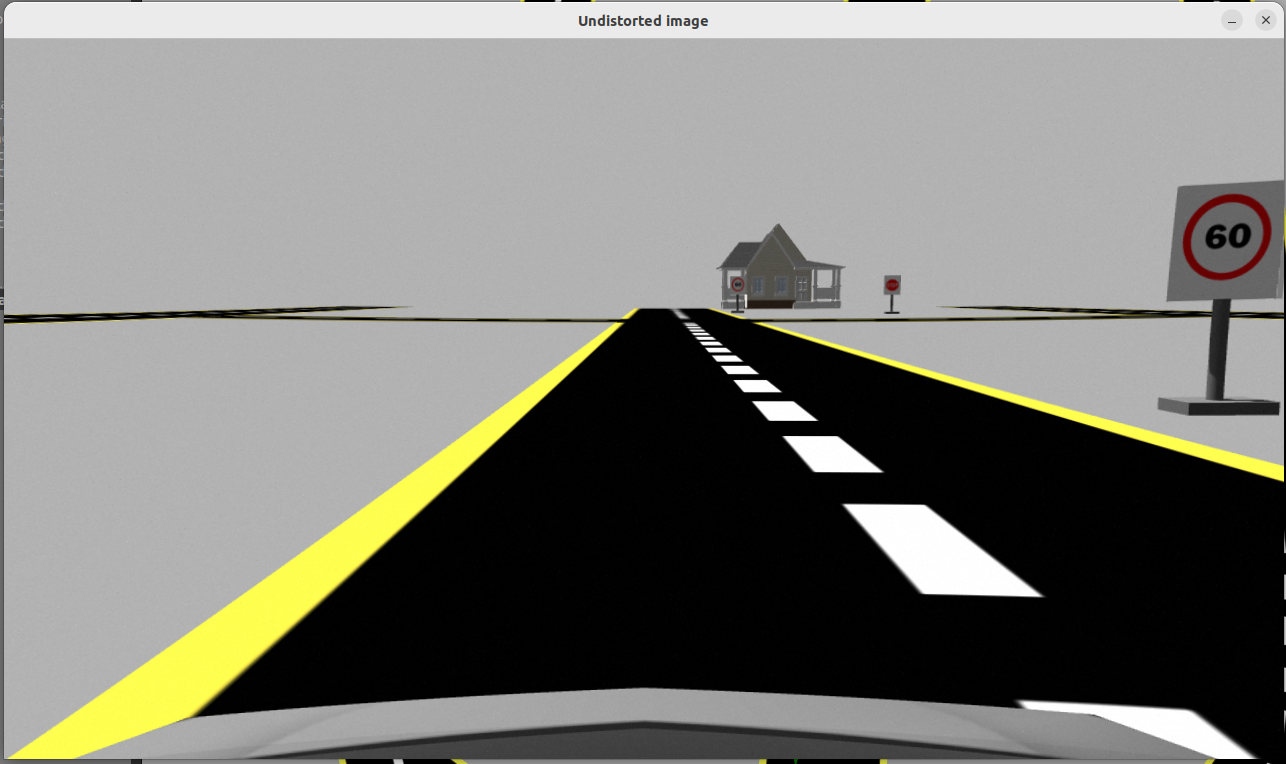
\includegraphics[width=0.6\linewidth]{images/3-lane/u._img.png}
    \caption{Sau hiệu chỉnh}
\end{figure}

\noindent Có thể ngay lúc này, khi nhìn vào bức ảnh đã được hiệu chỉnh, ta vẫn chưa thấy sự khác biệt quá lớn lao nào so với bức ảnh đầu vào, tuy nhiên việc này sẽ tăng hiệu quả cũng như độ chính xác trong việc áp dụng các giải thuật về sau.

\subsection{Phân ngưỡng ảnh}
\subsubsection{Edge và Gradient}
\subsubsection*{Edge}
Trong ảnh số, những điểm ảnh có cường độ ảnh sáng thay đổi mạnh so với các điểm xung quanh thường được gọi là các điểm cạnh (edge point). Cạnh (edge) là tập hợp các điểm cạnh tạo nên một hình dạng có ý nghĩa nào đó liên quan đến thông tin hình dạng và cấu trúc của đối tượng trong ảnh, ví dụ đường bao của một khuôn mặt, cấu trúc vành mũ, ... Tách cạnh là quá trình trích rút các thông tin tin cạnh bằng các phép toán xử lý ảnh.\\
Ví dụ như ta có một bức ảnh và ta lấy một đường kẻ ngang rồi ta sẽ lấy mức xác theo đường thằng đó, ta sẽ thấy được sự thay đổi mức xám ở các vị trí. \\

\begin{figure}[htbp]
    \centering
    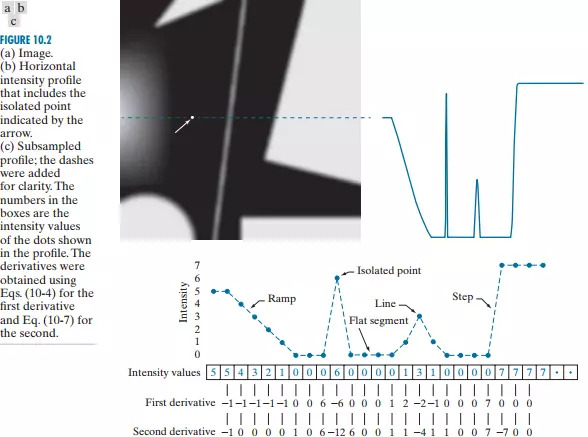
\includegraphics[width=0.5\linewidth]{images/3-lane/edge.jpg}
\end{figure}
\subsubsection*{Gradient}
Khi nhắc đến sự thay đổi đổi thì ta thường nhắc tới Gradient. Gradient của hàm cho biết hàm tăng mạnh như thế nào.\\
Ví dụ với hàm 1 chiều: $f(x) = x^2$ thì Gradient của nó được ký hiệu và tính như sau: $$\nabla f(x) = \frac{\partial f(x)}{\partial x} = 2x$$
\begin{itemize}
    \item Grad(2) = 4 chỉ ra hướng tăng của hàm là bên phải
    \item Grad (-1) = -2 chỉ ra hướng tăng của hàm nằm ở bên trái.
\end{itemize}
Gradient không chỉ tính bằng đạo hàm bậc 1, ta cũng thể tính bằng đạo hàm bậc. Với độ biến đổi của mức sáng bên trên ta tính được đạo hàm bậc 1, bậc 2 và công thức tương ứng như sau: 
\begin{figure}[htbp]
    \centering
    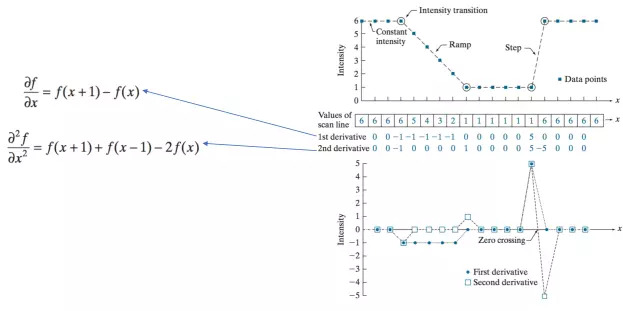
\includegraphics[width=0.5\linewidth]{images/3-lane/gradgrad.jpg}
\end{figure}
\newpage
\subsubsection{Phát hiện cạnh sử dụng đạo hàm}
Ta có bức ảnh đã được hiệu chỉnh trong phần trước:\\

\begin{figure}[htp]
    \centering
    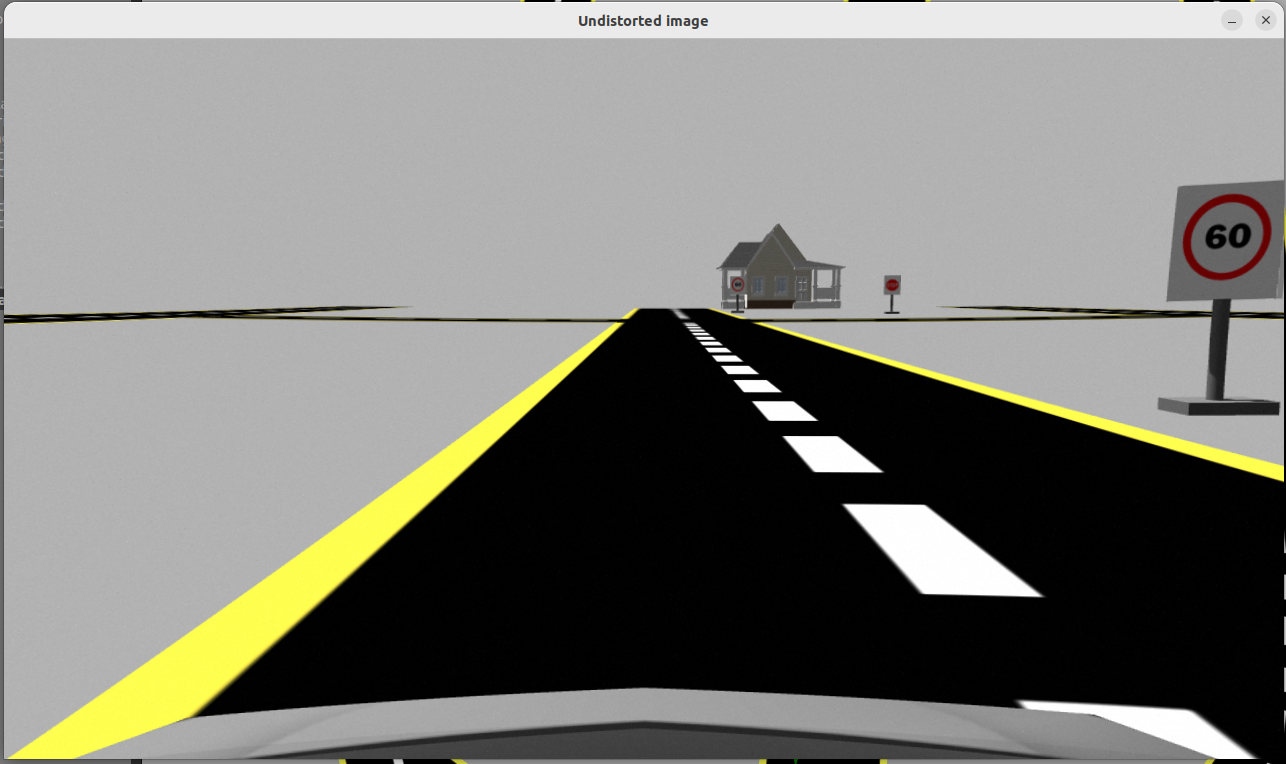
\includegraphics[width=0.4\linewidth]{images/3-lane/u._img.png}
    \caption{Ảnh đã hiệu chỉnh}
\end{figure}
\noindent Có thể sử dụng đạo hàm để phát hiện biên cạnh hoặc đường viền của làn đường trong hình ảnh, đặc biệt là khi màu sắc của đường và nền có sự tương phản cao. Trong hệ màu RGB, mỗi điểm ảnh có thể được biểu diễn bằng ba giá trị tương ứng với mức độ đỏ (R), xanh lá cây (G), và xanh dương (B). Sự thay đổi nhanh chóng trong giá trị này có thể tương ứng với sự thay đổi trong màu sắc, cho phép chúng ta phát hiện được các đường biên.

\noindent Một cách phổ biến để phát hiện cạnh là sử dụng đạo hàm của ảnh. Đạo hàm có thể được tính theo nhiều cách, nhưng một cách phổ biến là sử dụng bộ lọc Sobel hoặc Scharr. 

\noindent Như đã nói ở trên, có hai cách để phát hiện cạnh sử dụng đạo hàm:
\begin{itemize}
    \item Phát hiện giá trị cực tiểu hoặc cực đại địa phương trong đạo hàm bậc 1
    \item Phát hiện zero-crosssing (chính là chỗ giá trị từ âm sang dương hoặc ngược lại bạn có thể nhìn chú thích ở hình trên) trong đạo hàm bậc 2.
\end{itemize}

% \begin{figure}[htbp]
%     \centering
%     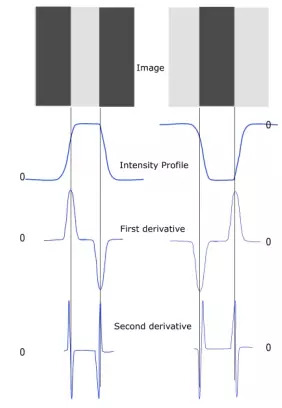
\includegraphics[width=0.3\linewidth]{images/3-lane/deri.jpg}
% \end{figure}

\noindent Đạo hàm trong không gian 2 chiều được tính như sau:
\[
    \nabla f(x,y) = \frac{\partial f(x,y)}{\partial x} \Vec{i} + \frac{\partial f(x,y)}{\partial y} \Vec{j}
\]
Tuy nhiên để áp dụng trong xử lí ảnh, việc xấp xỉ hóa đạo hàm của hàm rời rạc là cần thiết. Xấp xỉ đạo hàm bậc nhất hàm gradient được tính như sau (1), ở đây giá trị nhỏ nhất trong ảnh là 1 pixel:
\[
\frac{\partial f(x,y)}{\partial x} = f(x+1,y) - f(x,y)
\]
\[
\frac{\partial f(x,y)}{\partial y} = f(x,y+1) - f(x,y)
\]
Độ lớn của gradient cho biết cường độ của cạnh tại điểm đó:
\[
|\nabla f(x,y)| = \sqrt{\left( \frac{\partial f(x,y)}{\partial x}\right)^2 + \left(\frac{\partial f(x,y)}{\partial y}\right)^2}
\]
Trong xử lí ảnh, ta có các bước để tính gradient như sau:
\begin{itemize}
    \item Gradient theo cột
    \item Gradient theo hàng
    \item tổng hợp hai Gradient trên
\end{itemize}
Nếu chúng ta sử dụng phương pháp thông thường để tính gradient bằng cách duyệt từng hàng và cột của ma trận, quá trình này thường mất nhiều thời gian tính toán. Để tối ưu hóa quá trình này, có một số phương pháp và kỹ thuật hiện đại mà chúng ta có thể áp dụng.\\
Một trong những cách là sử dụng phép tính gradient thông qua các phép toán ma trận và kernel mà chúng ta đã học từ bài trước. Thay vì duyệt qua từng phần tử của ma trận và tính gradient riêng lẻ, chúng ta có thể sử dụng các phép toán ma trận để thực hiện tính toán này một cách hiệu quả hơn.\\
Cụ thể, ta có thể sử dụng phép tích chập (convolution) với kernel đã được học trước đó để áp dụng tính toán gradient cho toàn bộ ma trận một cách đồng thời. Điều này giúp giảm thiểu số lượng phép toán cần thực hiện và tăng tốc quá trình tính gradient.\\
Với việc sử dụng phép toán kernel và kỹ thuật convolution, chúng ta không chỉ giảm thời gian tính toán mà còn tận dụng được hiệu suất của các thư viện và trình tối ưu hóa ma trận hiện đại, giúp tăng cường khả năng tính toán của thuật toán gradient trong bài toán của chúng ta.

\subsubsection{Áp dụng phương pháp để phân ngưỡng ảnh}
Có khá nhiều kernel thông dụng được sử dụng cho việc phát hiện biên và cạnh, cũng như có một số phương pháp hiện đại có thể dùng cho việc này(có thể kể đến giải thuật Canny), nhóm nhận định rằng với tính chất cũng như yêu cầu về sự cân bằng giữa tốc độ xử lí và độ chính cao cao, nên sẽ chọn \textbf{Sobel kernel}, vừa đơn giản hóa các thông tin mà máy chủ cần xử lí, đồng thời vẫn đảm bảo được độ chính xác cao.\\
Sobel kernel:
\[\frac{1}{4}
\left[
    \begin{array}{ccc}
        1 & 0 & -1  \\
        2 & 0 & -2 \\
        1 & 0 & -1
    \end{array}
\right]
\]

Như vạy, sau khi xử dụng Sobel kernel để lọc bức ảnh đầu vào, ta thu được:

\begin{figure}[htbp]
    \centering
    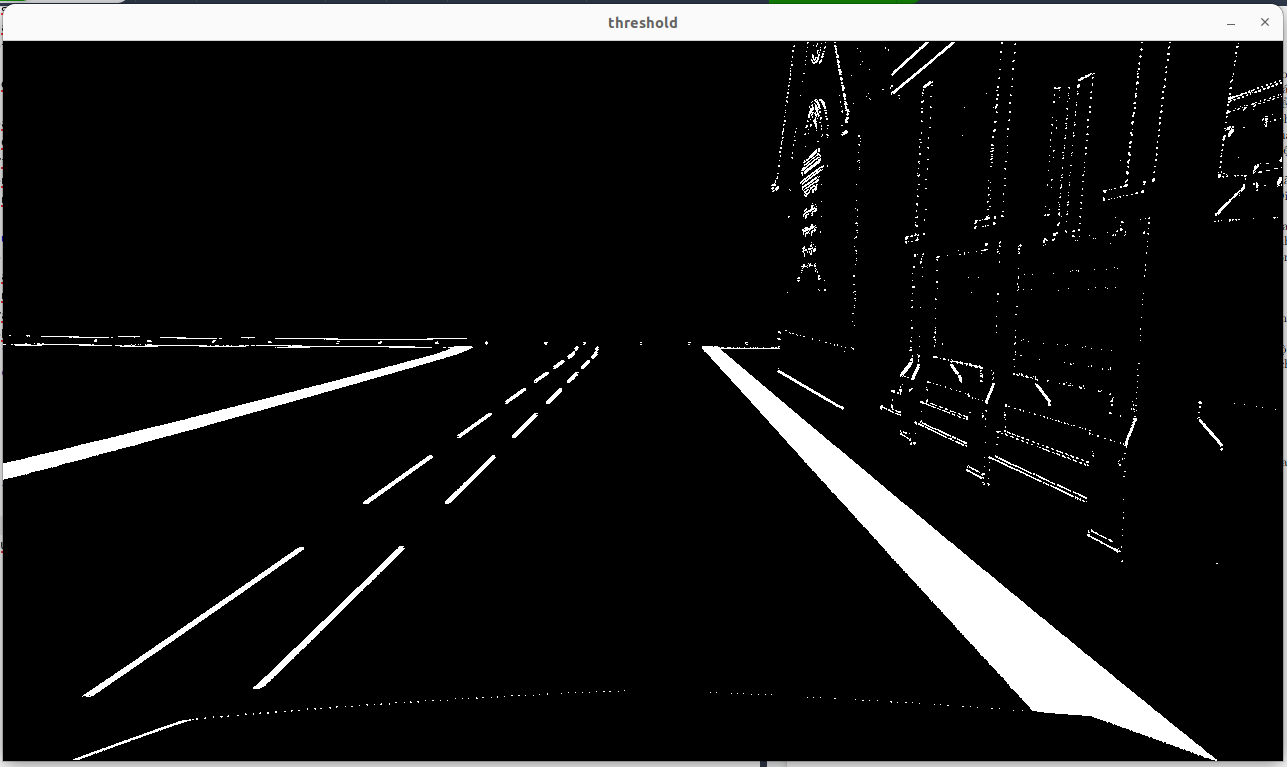
\includegraphics[width=0.8\linewidth]{images/3-lane/threshold.png}
    \caption{Phân ngưỡng ảnh}
\end{figure}

Với việc làn đường màu trắng và vàng, là những màu có cường độ lớn, ta đã thu được hình ảnh trong đó những đường kẻ nối liền bên tay phải và các đường nét đứt bên trái đều là cạnh và làn đường mà ta đã phát hiện được.

\subsection{Chuyển góc nhìn (get perspective transform)}
Tiếp theo, ta sẽ tiến hành việc thay đổi góc nhìn của ô tô đối với làn đường. Ta cũng thấy, trong hình ảnh mà camera thu nhận, làn đường không phải là hai đường thẳng song song mà lại là hai đường thẳng giao nhau ở phía xa của bức ảnh. Như vậy, việc đánh giá tính chất của làn đường (thẳng, cong trái, phải ..) là rất khó khắn, vì vậy ta sẽ tiến hành chuyển đổi góc nhìn của ô tô sang như thể đang nhìn vuông góc từ trên trời xuống.\\
Các bước được dùng để tiến hành đổi góc nhìn như sau:
\begin{enumerate}
    \item Chọn ma trận đến, ma trận đích 
    \item Tính toán ma trận dùng để biến đổi từ ma trận đầu thành ma trận cuối và ngược lại (sử dụng \textbf{cv2.getPerspectiveTransform}
    \item Thay đổi bức ảnh đầu vào bằng \textbf{cv2.warpPerspective} và xuất ra kết quả.
\end{enumerate}
Lưu ý, vì ta đang xử lí trên ảnh nên ma trận bốn điểm là một ma trận 4 x 2 vì đây là không gian 2D. Đồng thời các điểm này phải nằm trong độ lớn giới hạn của khung hình là 1280 x 720 (pixel). Sau khi thực thi ta thu được kết quả sau:\\
%
Với bức ảnh đầu vào:\begin{figure}[htbp]
    \centering
    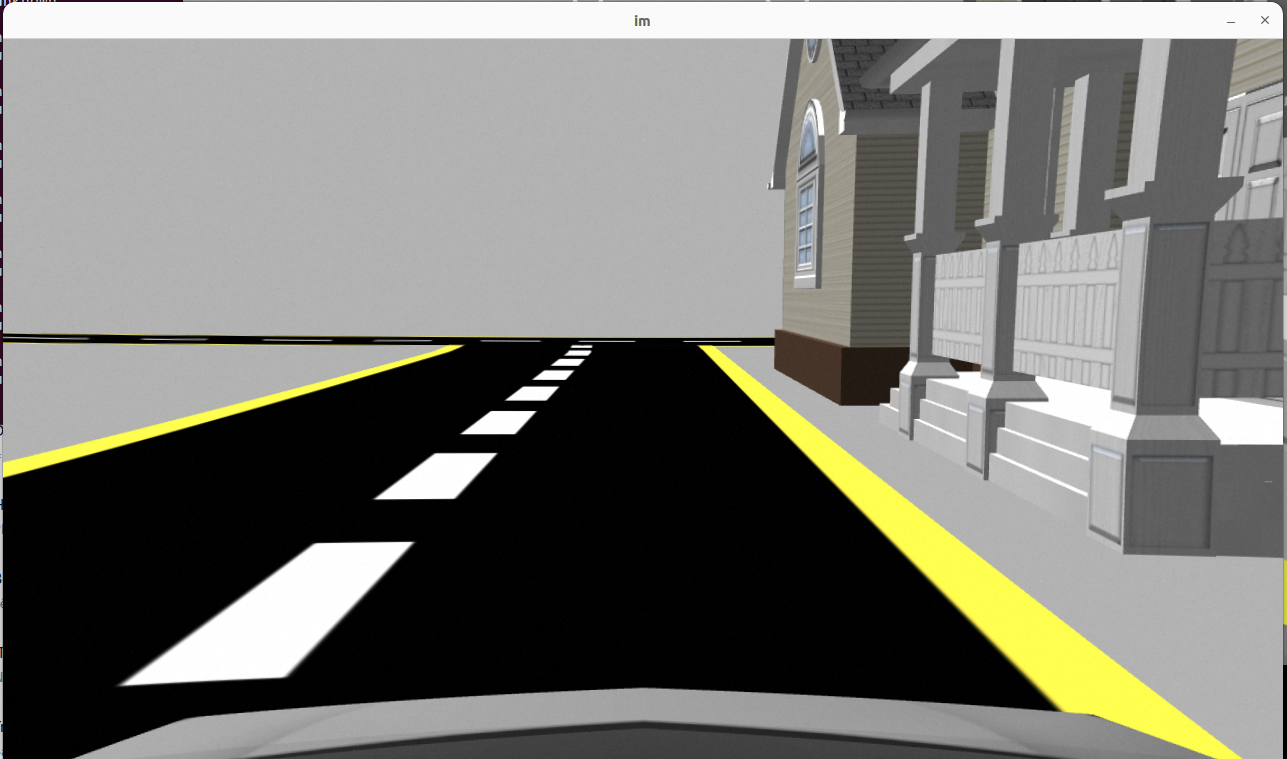
\includegraphics[width=0.4\linewidth]{images/3-lane/ori.png}
    \caption{Đầu vào}
\end{figure}
ta được:
\begin{figure}[htbp]
    \centering
    \subfigure[]{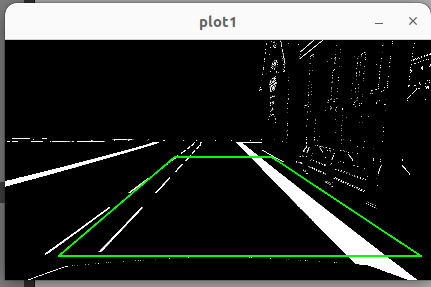
\includegraphics[width=0.4\linewidth]{images/3-lane/plot1.png}}
    \subfigure[]{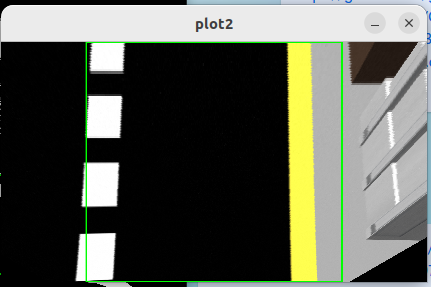
\includegraphics[width=0.4\linewidth]{images/3-lane/plot2.png}}
    \caption{Đổi góc nhìn}
\end{figure}

\noindent Như vậy, giải thuật thay đổi tầm nhìn của ô tô, cộng với việc đã phân ngưỡng ảnh trước đó, bức ảnh thu được gần như đã hiển thị rõ phàn mà ta gọi là làn đường cũng như loại bỏ những thông tin không cần thiết về các vật thể khác nhau xuất hiện trên đường. Tiếp theo ta sẽ sử dụng một số phép tính toán để có thể vẽ ra một đường thẳng (hoặc cong) có thế chưa gần hết từng bên của làn đường dể có thể thực hiện tính toán cân bằng. 

\subsection{Nhận diện làn đường}
Có thể thấy được trên hình, phần làn đường không chỉ đơn giản là những pixel đơn rời rạc được nối lại với nhau tạo thành một đường thẳng hay cong, mà bao gồm một vùng pixel gồm các pixel có độ lớn tương đồng nhau. Để có thể vẽ ra được một làn đường phù hợp, ta sẽ sử dụng phương pháp của sổ trượt (sliding window search). Tóm tắt quy trình sử dụng phương pháp này như sau:
\begin{enumerate}
    \item \textbf{Chia ảnh thành các cửa sổ nhỏ:}\\ Hình ảnh được chia thành các cửa sổ (window) nhỏ có kích thước cố định hoặc biến đổi được. Mỗi cửa sổ đại diện cho một vùng nhỏ trên hình ảnh.
    \item \textbf{Duyệt qua từng cửa sổ:}\\ Các cửa sổ được duyệt qua từ trái sang phải và từ trên xuống dưới hoặc theo hướng khác nhau tùy thuộc vào chiều của sliding window. Mỗi cửa sổ được đưa vào một mô hình hoặc bộ phân loại để kiểm tra xem nó có chứa đối tượng quan tâm hay không.
    \item \textbf{Xác định vị trí của đối tượng:}\\ Khi một cửa sổ được đưa vào mô hình và được phân loại, vị trí của nó trên hình ảnh được xác định. Các cửa sổ được di chuyển tiếp theo và quá trình lặp lại cho đến khi toàn bộ hình ảnh được duyệt qua.
    \item \textbf{Tối ưu hóa và loại bỏ cửa sổ không cần thiết:}\\ Đối với hiệu suất tốt hơn, có thể thực hiện các kỹ thuật tối ưu hóa như sử dụng các kỹ thuật quét tăng cường (e.g., image pyramid) để giảm số lượng cửa sổ cần xem xét.
    
\end{enumerate}
Sau khi sử dụng qui trình trên, hình ảnh đường thẳng (hoặc cong) được dùng để fit với mỗi làn đường sẽ có dạng như sau:
\begin{figure}[htbp]
    \centering
    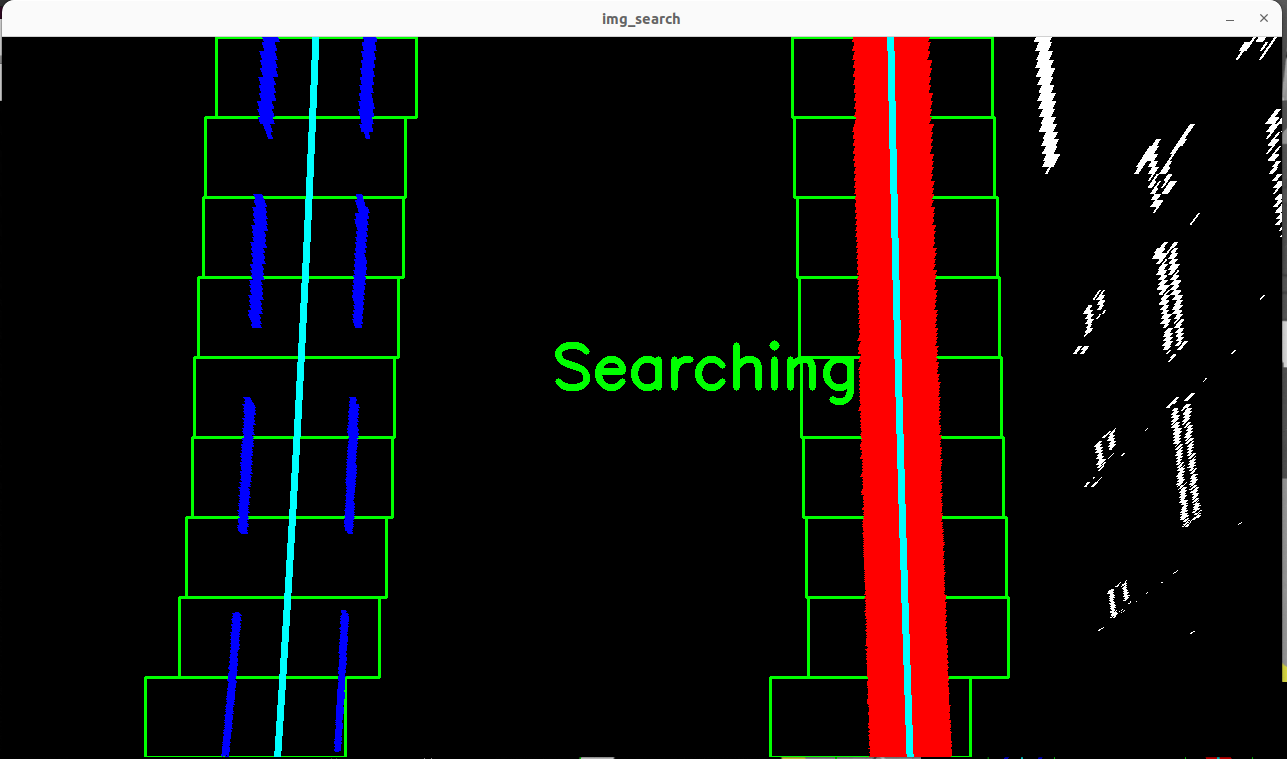
\includegraphics[width=0.6\linewidth]{images/3-lane/sliding.png}
    \caption{Nhận diện làn đường}
\end{figure}
\subsection{Tổng hợp}
Như vậy, sau khi có được thông tin của các đường thẳng (hoặc cong) fit với hai làn đường, từ đó ta sẽ sử dụng chúng để tính toán các thông số tiếp theo như là độ cong của mỗi làn, khoảng cách của xe với trung tâm của làn, ta cũng sẽ vẽ 1 đường nhầm thể hiện xu hướng rẽ trung bình của hai làn đường để biết rằng đường đang thẳng hay cong sang trái(phải).... Đồng thời ta sẽ để output chứa tất cả các hình ảnh của các bước trên với mục đích xe sẽ phải quản lí chặt chẽ các thông tin đó cũng như dễ dàng hơn cho việc debug sau này.\\
Ta thu được:
\begin{figure}[htbp]
    \centering
    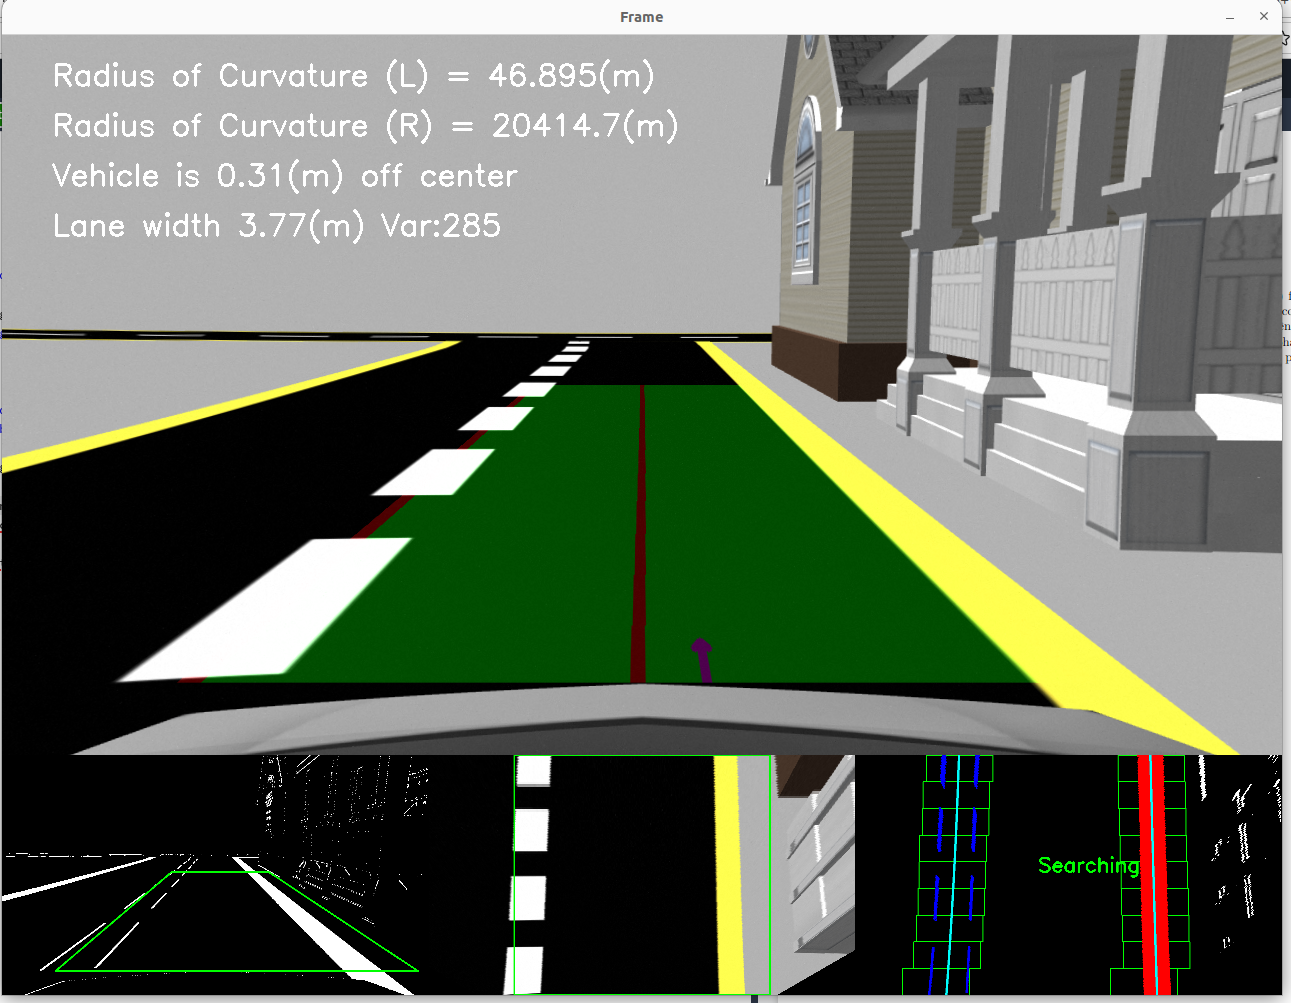
\includegraphics[width=0.8\linewidth]{images/3-lane/combine.png}
    \caption{Tổng hợp thông tin}
\end{figure}